\begin{question}
\noindent Triangle $L$ has vertices $A(1,0)$, $B(3,0)$ and $C(3,2)$, as shown on the grid.

\begin{center}
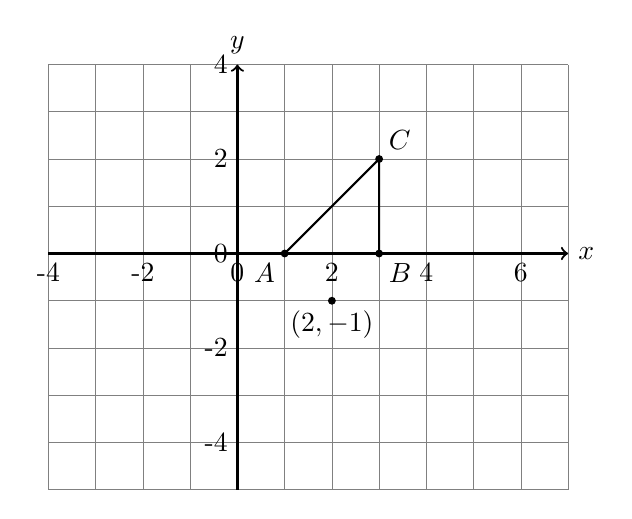
\begin{tikzpicture}[scale=0.6]
    \draw[step=1cm, gray, very thin] (-4,-5) grid (7,4);
    \draw[thick,->] (-4,0) -- (7,0) node[right]{$x$};
    \draw[thick,->] (0,-5) -- (0,4) node[above]{$y$};

    \foreach \x in {-4,-2,0,2,4,6}
        \node[below] at (\x,0) {\x};
    \foreach \y in {-4,-2,0,2,4}
        \node[left] at (0,\y) {\y};

    % Triangle L
    \draw[thick] (1,0) -- (3,0) -- (3,2) -- cycle;
    \filldraw (1,0) circle (2pt) node[below left]{$A$};
    \filldraw (3,0) circle (2pt) node[below right]{$B$};
    \filldraw (3,2) circle (2pt) node[above right]{$C$};

    % Centre of rotation
    \filldraw (2,-1) circle (2pt) node[below]{$(2,-1)$};
\end{tikzpicture}
\end{center}

\noindent Rotate triangle $L$ by $180^{\circ}$ about the point $(2,-1)$.

\noindent Draw the image of triangle $L$ and label it $L'$.

\vspace{6cm}

\begin{flushright}
    \answerplain{3}
\end{flushright}
\end{question}